%ju 28-Mai-22 03-Grundlagen-Elektrik2.tex
\section{Potentialbestimmung}\label{potentialbestimmung}

\begin{figure}[!ht]% hier: !ht
\centering
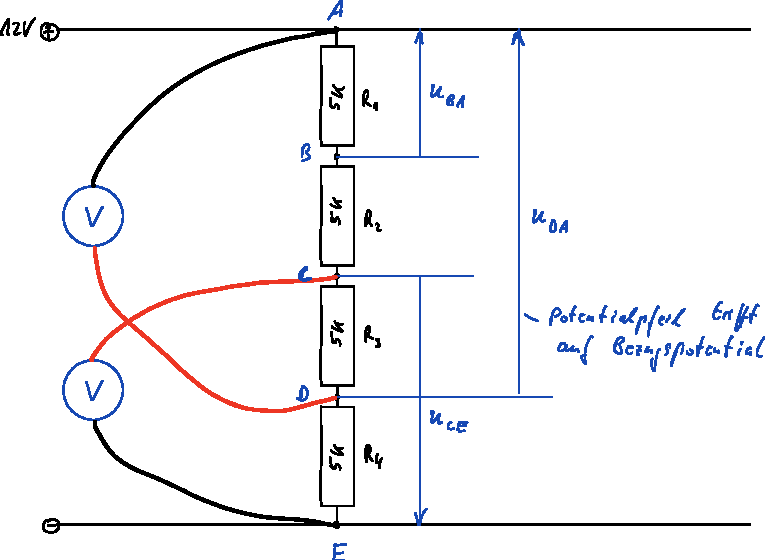
\includegraphics[width=0.6\textwidth]{images/Skizze/28_FT_Potentialbestimmung.pdf}
\caption{Potentialbestimmung}
%\label{fig:}%% anpassen
\end{figure}

Klemmenspannung und Potential

\begin{itemize}
\item
  $U_{R_1} = 3~V$, $U_{R_3} = 3~V$
\item
  $U_{CE} = 6~V$, $U_{BA} = -3~V$, $U_{DA} = -9~V$
\end{itemize}

Möchte man das/ein Potential an einem Punkt in einem Stromkreis
messen/bestimmen, bezieht man sich immer auf ein Bezugspotenzial. Die
Schreibweise dieser Messung lautet dann zum Beispiel $U_{CE}$, hierbei
möchte ich also das Potential C messen, C ist der erste Buchstabe, an
ihm wird der \emph{rote Clip} des Multimeters angeschlossen. Das
Bezugspotenzial hierbei E ist der zweite Buchstabe, hier wird
grundsätzlich der \emph{schwarze Clip} des Multimeters angeschlossen.
Potentialbestimmungen können auch zeichnerisch dargestellt werden.
Hierbei lautet die Vereinbarung, die Pfeilspitze des Spannungs- oder
Potentialpfeils trifft immer auf das Bezugspotenzial. Beispiel
$U_{DA}$.

\newpage

\section{Brückenschaltung -
Brückenspannung}\label{brueckenschaltung-brueckenspannung}

\begin{figure}[!ht]% hier: !ht
\centering
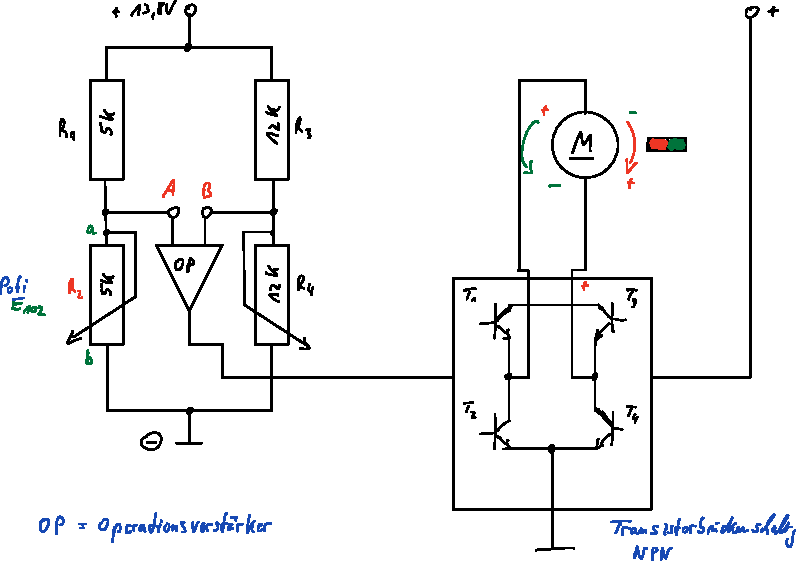
\includegraphics[width=0.6\textwidth]{images/Skizze/28_FT_Brueckenschaltung.pdf}
\caption{Brückenschaltung}
%\label{fig:}%% anpassen
\end{figure}

$U_{A\text{-}} = 6,9~V$, $U_{B\text{-}} = 6,9~V$, $U_{AB} = 0~V$
(keine Differenz)

$U_{A\text{+}} = -6,9~V$, $U_{B\text{+}} = -6,9~V$, $U_{AB} = 0~V$
(keine Differenz)

Poti $\to R_2 = 1~k$

$I_{Li} = \frac{U_{ges}}{R_{{Li}_{ges}}} = \frac{U_{ges}}{R_1 + R_2} = \frac{13,8}{5000 + 1000} =0,0023~A$

$U_{R_1} = R_1 \cdot I_{Li} = 5000~\Omega \cdot 0,0023~A = 11,5~V$

$U_{A\text{+}} = -11,5~V$, $U_{B\text{+}} = -6,9~V$,
$U_{AB} = -4,6~V$

$I_{Re} = \frac{U_{R_3}}{R_3} = \frac{11,5}{12000} =0,00096~A$

$R_4 = \frac{U_{R_4}}{I_{Re}} = \frac{U_{ges} - U_{R_3}}{I_{Re}} = \frac{13,8 - 11,5}{0,00096} = 2395,83~\Omega$

\newpage

\section{Signalanlage Oldtimer
(Prüfung)}\label{signalanlage-oldtimer-pruefung}

\textbf{Aufgabe:} Stromlaufplan zeichnen

Ein Kunde beanstandet Folgendes:

\textbf{>>Wenn ich den Fahrtrichtungsanzeiger setze und dabei das
Bremspedal betätige, bleibt mein Fahrtrichtungsanzeiger stehen.<<}

Lösen Sie dieses Problem mit einem entsprechenden Relaisschaltung.
Komponenten, die vorhanden sein müssen: Batterie, 30/15/31ger Schiene,
Blinkrelais (2-polig), Kontrollleuchte, Blinkerschalter, zwei
Blinkleuchten links, zwei Blinkleuchten rechts. Dazu ein entsprechendes
Relais.

\textbf{Problem - Spannungsverlust durch Bremse treten}

\begin{figure}[!ht]% hier: !ht
\centering
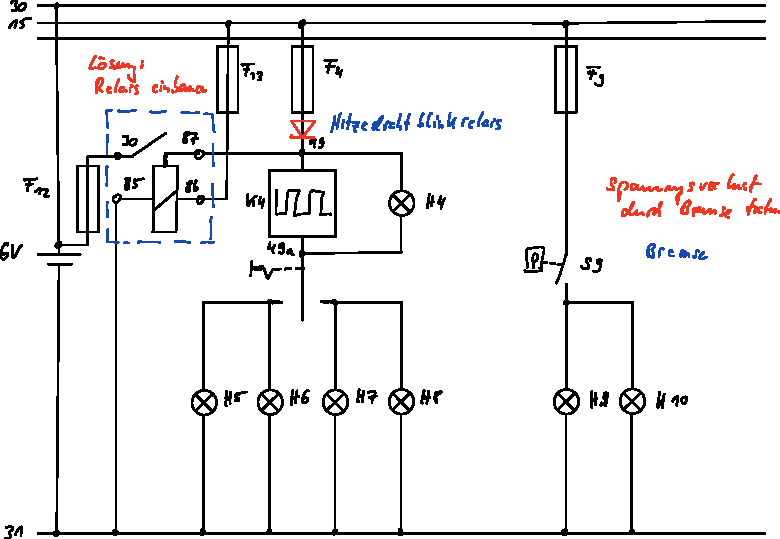
\includegraphics[width=0.9\textwidth]{images/Skizze/29_FT_Signalanlage_Relais_6V.pdf}
\caption{Signalanlage Oldtimer Relais}
%\label{fig:}%% anpassen
\end{figure}

\emph{Lösung} $\to$ Relais einbauen.

\emph{Zündung Einschalten} Steuerstrom baut magnetisches Feld auf und
schneidet die Spule, induziert dabei eine Spannung von $6~V$.

\textbf{Blinkfrequenz} $90 \pm30$ Impulse pro Minute

\emph{Zündung ausschalten} Diode einbauen zwischen F4 und Anschluß 49

\newpage

\section{Tagfahrlicht verdrahten mit Relais Öffner oder
Schließer}\label{tagfahrlicht-verdrahten-mit-relais-oeffner-oder-schliesser}

\textbf{Vorteile LED}

\begin{itemize}
\item
  Stromverbrauch
\item
  Haltbarkeit
\item
  Bezeichnung >>RL<<
\item
  Abstand $600~mm$
\end{itemize}

\begin{figure}[!ht]% hier: !ht
\centering
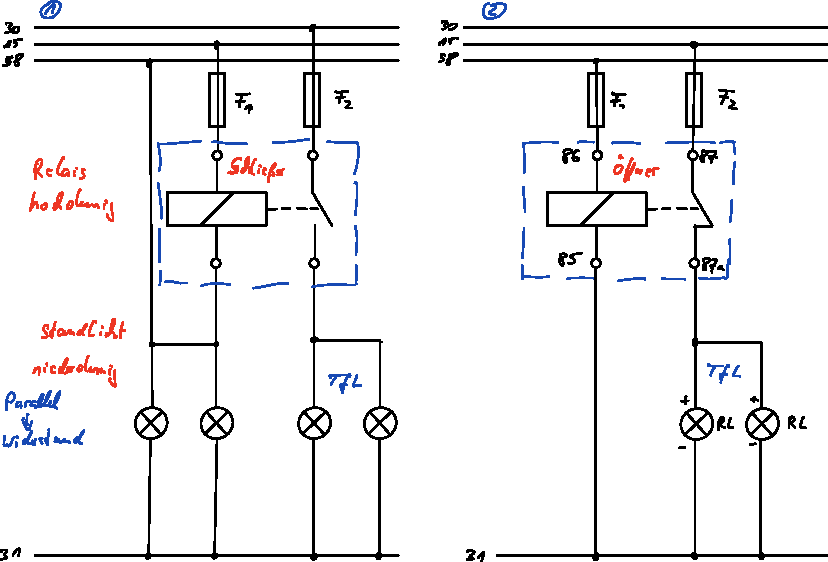
\includegraphics[width=0.9\textwidth]{images/Skizze/29_FT_Tagfahrlicht_Relais.pdf}
\caption{Tagfahrlicht Relais}
%\label{fig:}%% anpassen
\end{figure}

\textbf{1) Wieso leuchtet das Tagfahrlicht ohne Standlicht?} - Das
Relais ist hochohmig und das Standlicht (4x Lampen parallel) ist
niederohmig. - Das Relais holt sich die Masse über die Lampen.

\textbf{2) Was muss ich machen, damit ich Kraftstoff einsparen kann?} -
Vgl. Abb. Tagfahrlicht - (1) Sicherung \emph{F1} ziehen - (2) Sicherung
\emph{F1} und \emph{F2} ziehen

\newpage

\section{Elektromotorarten}\label{elektromotorarten}

\subsection{Nebenschlussmotor}\label{nebenschlussmotor}

Urmotor im Kfz, außer Starter

\begin{table}[!ht]% hier: !ht 
\centering 
	\caption{}% \label{tab:}%% anpassen 
\begin{tabular}{@{}ll@{}}
\hline
\textbf{Abk.} & \textbf{Bezeichnung} \\
\hline
$AW$ & Ankerwicklung (Spule) \\
$NSW$ & Nebenschlusswicklung (Spule) \\
$I_A$ & Ankerstrom \\
$I_{NSW}$ & Stromfluss durch die NSW \\
$RSW$ & Reihenschlusswicklung \\
$I_{RSW}$ & Stromfluss durch die RSW \\
\hline
\end{tabular} 
\end{table}

\textbf{a) Nebenschlussmotor mit Feldwicklung}

Kennlinie - Drehzahlverhalten

\begin{figure}[!ht]% hier: !ht
\centering
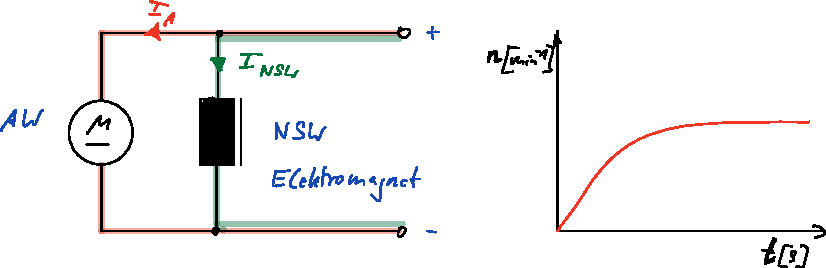
\includegraphics[width=0.6\textwidth]{images/Skizze/30_FT_Nebenschlussmotor_mit_Feldwicklung.pdf}
\caption{Nebenschlussmotor mit Feldwicklung}
%\label{fig:}%% anpassen
\end{figure}

\textbf{b) Nebenschlussmotor mit Permanenterregung}

Kennlinie - Drehzahlverhalten

\begin{figure}[!ht]% hier: !ht
\centering
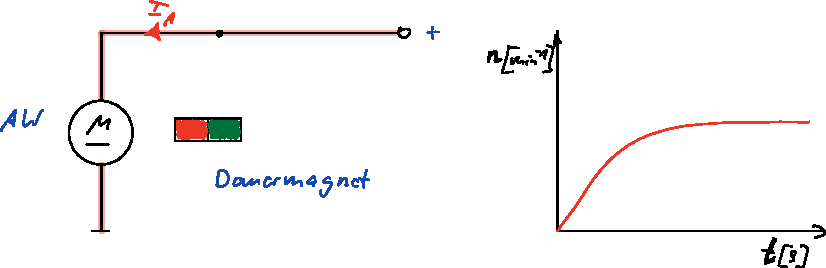
\includegraphics[width=0.6\textwidth]{images/Skizze/30_FT_Nebenschlussmotor_mit_Permanenterregung.pdf}
\caption{Nebenschlussmotor mit Permanenterregung}
%\label{fig:}%% anpassen
\end{figure}

\subsection{Reihenschlussmotor}\label{reihenschlussmotor}

Dreht hoch

Kennlinie - Drehzahlverhalten

\begin{figure}[!ht]% hier: !ht
\centering
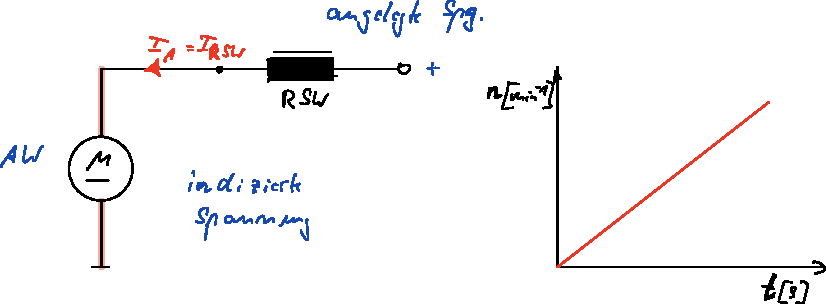
\includegraphics[width=0.6\textwidth]{images/Skizze/30_FT_Reihenschlussmotor.pdf}
\caption{Reihenschlussmotor}
%\label{fig:}%% anpassen
\end{figure}

\subsection{Doppelschlussmotor}\label{doppelschlussmotor}

Hohe Leistung

Kennlinie - Drehzahlverhalten

\begin{figure}[!ht]% hier: !ht
\centering
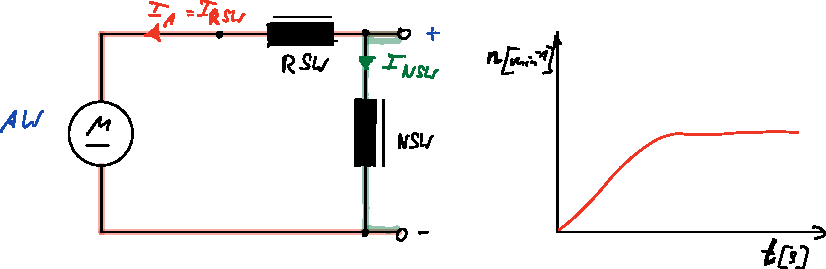
\includegraphics[width=0.6\textwidth]{images/Skizze/30_FT_Doppelschlussmotor.pdf}
\caption{Doppelschlussmotor}
%\label{fig:}%% anpassen
\end{figure}

\subsection{Wechselstrommotor}\label{wechselstrommotor}

Kennlinie - Drehzahlverhalten

\begin{figure}[!ht]% hier: !ht
\centering
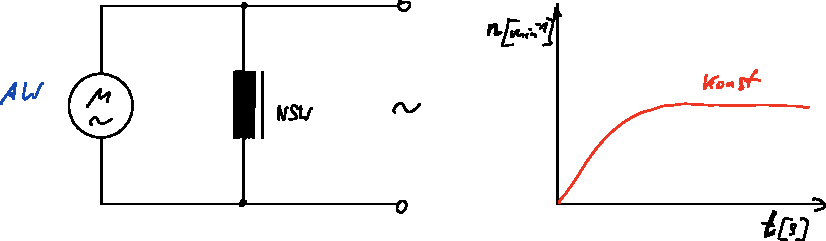
\includegraphics[width=0.6\textwidth]{images/Skizze/30_FT_Wechselstrommotor.pdf}
\caption{Wechselstrommotor}
%\label{fig:}%% anpassen
\end{figure}

\subsection{Schrittmotor}\label{schrittmotor}

Anwendung: Sitzverstellung, Scheinwerferhöhenverstellung, Schiebedach

Kennlinie - Drehzahlverhalten

\begin{figure}[!ht]% hier: !ht
\centering
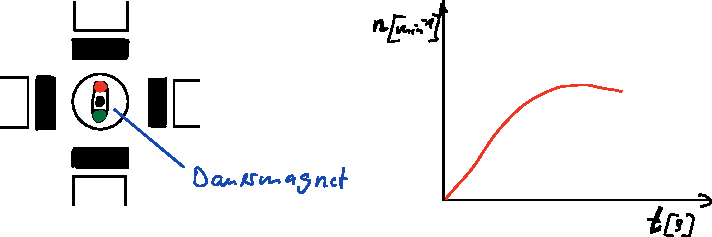
\includegraphics[width=0.6\textwidth]{images/Skizze/30_FT_Schrittmotor.pdf}
\caption{Schrittmotor}
%\label{fig:}%% anpassen
\end{figure}

\subsection{Drehstrommotor}\label{drehstrommotor}

Dozentenwechsel \ldots{}
